\documentclass[a4paper, 12pt]{article}

% srpski jezik, utf8
\usepackage[serbian]{babel}
\usepackage[utf8]{inputenc}

% podrska za graficke elemente
\usepackage{graphicx}

% podrska za boje
\usepackage{xcolor}

% podrska za stavljanje hyperlink-ova u sadrzaj
\usepackage{hyperref} 
\hypersetup{
	colorlinks	= true,
	citecolor	= gray,
	linkcolor	= blue
}

% podesavanja fonta
\newcommand{\thefont}{Myriad Pro}

\usepackage{mathspec}
\setmathsfont(Digits)[Numbers={Lining,Proportional}]{\thefont}
\setmathsfont(Latin)[Numbers={Lining,Proportional}]{\thefont}
\setmathsfont(Greek)[Numbers={Lining,Proportional}]{\thefont}
\setmathrm{\thefont}

\usepackage{polyglossia}
\setmainlanguage[Script=Latin]{serbian}
\setotherlanguage{english}
\newfontfamily{\serbianfont}[Script=Latin, Language=Serbian]{\thefont}
\newfontfamily{\serbianfonttt}{\thefont}
\newfontfamily{\englishfont}[Language=English]{\thefont}
\newfontfamily{\englishfonttt}{\thefont}

% za [H] u figure
\usepackage{float} 

% informacije o tekstu
\author{Ajzenhamer Nikola\\Bukurov Anja\\Vojislav Stankovi\'c}
\title{INFORMACIONI SISTEM NACIONALNE SLU\v ZBE ZA ZAPO\v SLJAVANJE}
\date{\today}

\begin{document}

\maketitle
\tableofcontents
\newpage

\section{Uvod}

Ovaj rad se bavi modeliranjem dela sistema Nacionalne slu\v zbe za zapo\v sljavanje republike Srbije. U okviru ovog rada, obra\' cena je pa\v znja i na mogu\' ca unapre\dj enja sistema.\\

Rad je izra\dj en kao timski studentski projekat na Matemati\v ckom fakultetu, na studijskom programu Informatika, prve godine Master studija. Projekat je odra\dj en pod nadzorom profesora dr Sa\v se Malkova, u okviru predmeta Informacioni sistemi.\\

U nastavku \' cemo detaljnije opisati rad Nacionalne slu\v zbe.

\subsection{Nacionalna slu\v zba za zapo\v sljavanje}

Nacionalna slu\v zba za zapo\v sljavanje (u daljem tekstu Nacionalna slu\v zba) obavlja poslove zapo\v sljavanja, osiguranja za slu\v caj nezaposlenosti, ostvarivanje prava iz osiguranja za slu\v caj nezaposlenosti i druga prava u skladu sa zakonom, odnosno poslove vo\dj enja evidencija u oblasti zapo\v sljavanja, kao i stru\v cno-organi\-zacione, upravne, ekonomsko-finansijske i druge op\v ste poslove u oblasti zapo\v sljavanja i osiguranja za slu\v caj nezaposlenosti, u skladu sa zakonom, svojim statutom i drugim aktima Nacionalne slu\v zbe.

\begin{mylandscape}
	\subsubsection{Dijagram konteksta}
	
	\begin{figure}[H]
		\centering
		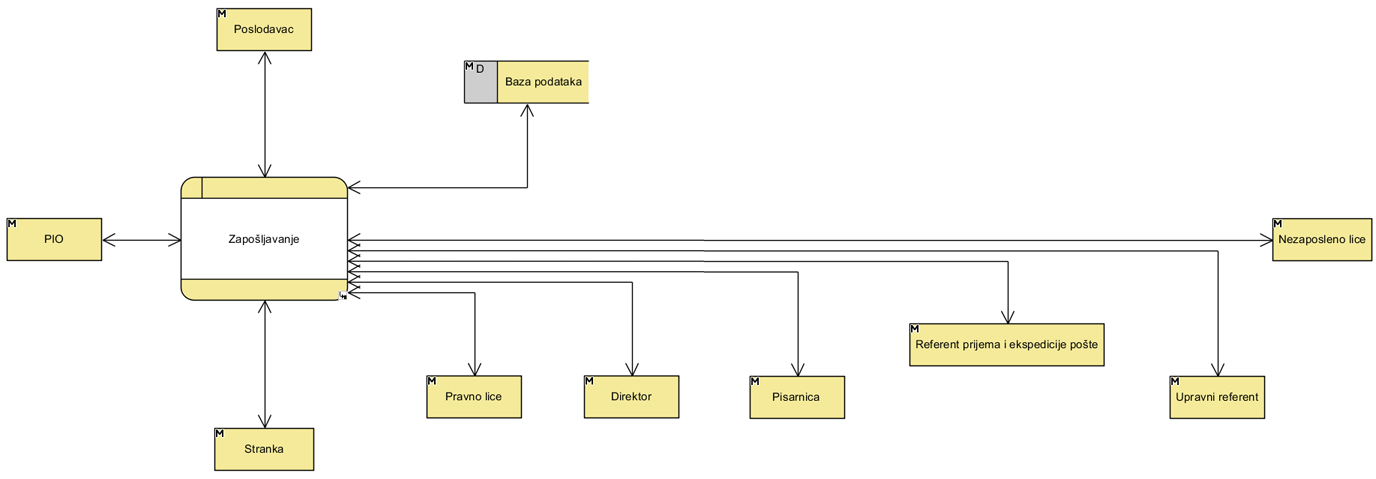
\includegraphics[width=0.8\paperwidth]{dijagrami/dijagrami-toka-podataka/zaposljavanje-dijagram-konteksta.png}
		\caption{Dijagram konteksta — prikaz sistema kao proces ''Zapo\v sljavanje''.}
		\label{dtp: dijagram konteksta}
	\end{figure}

	\newpage
	
	\begin{figure}[H]
		\centering
		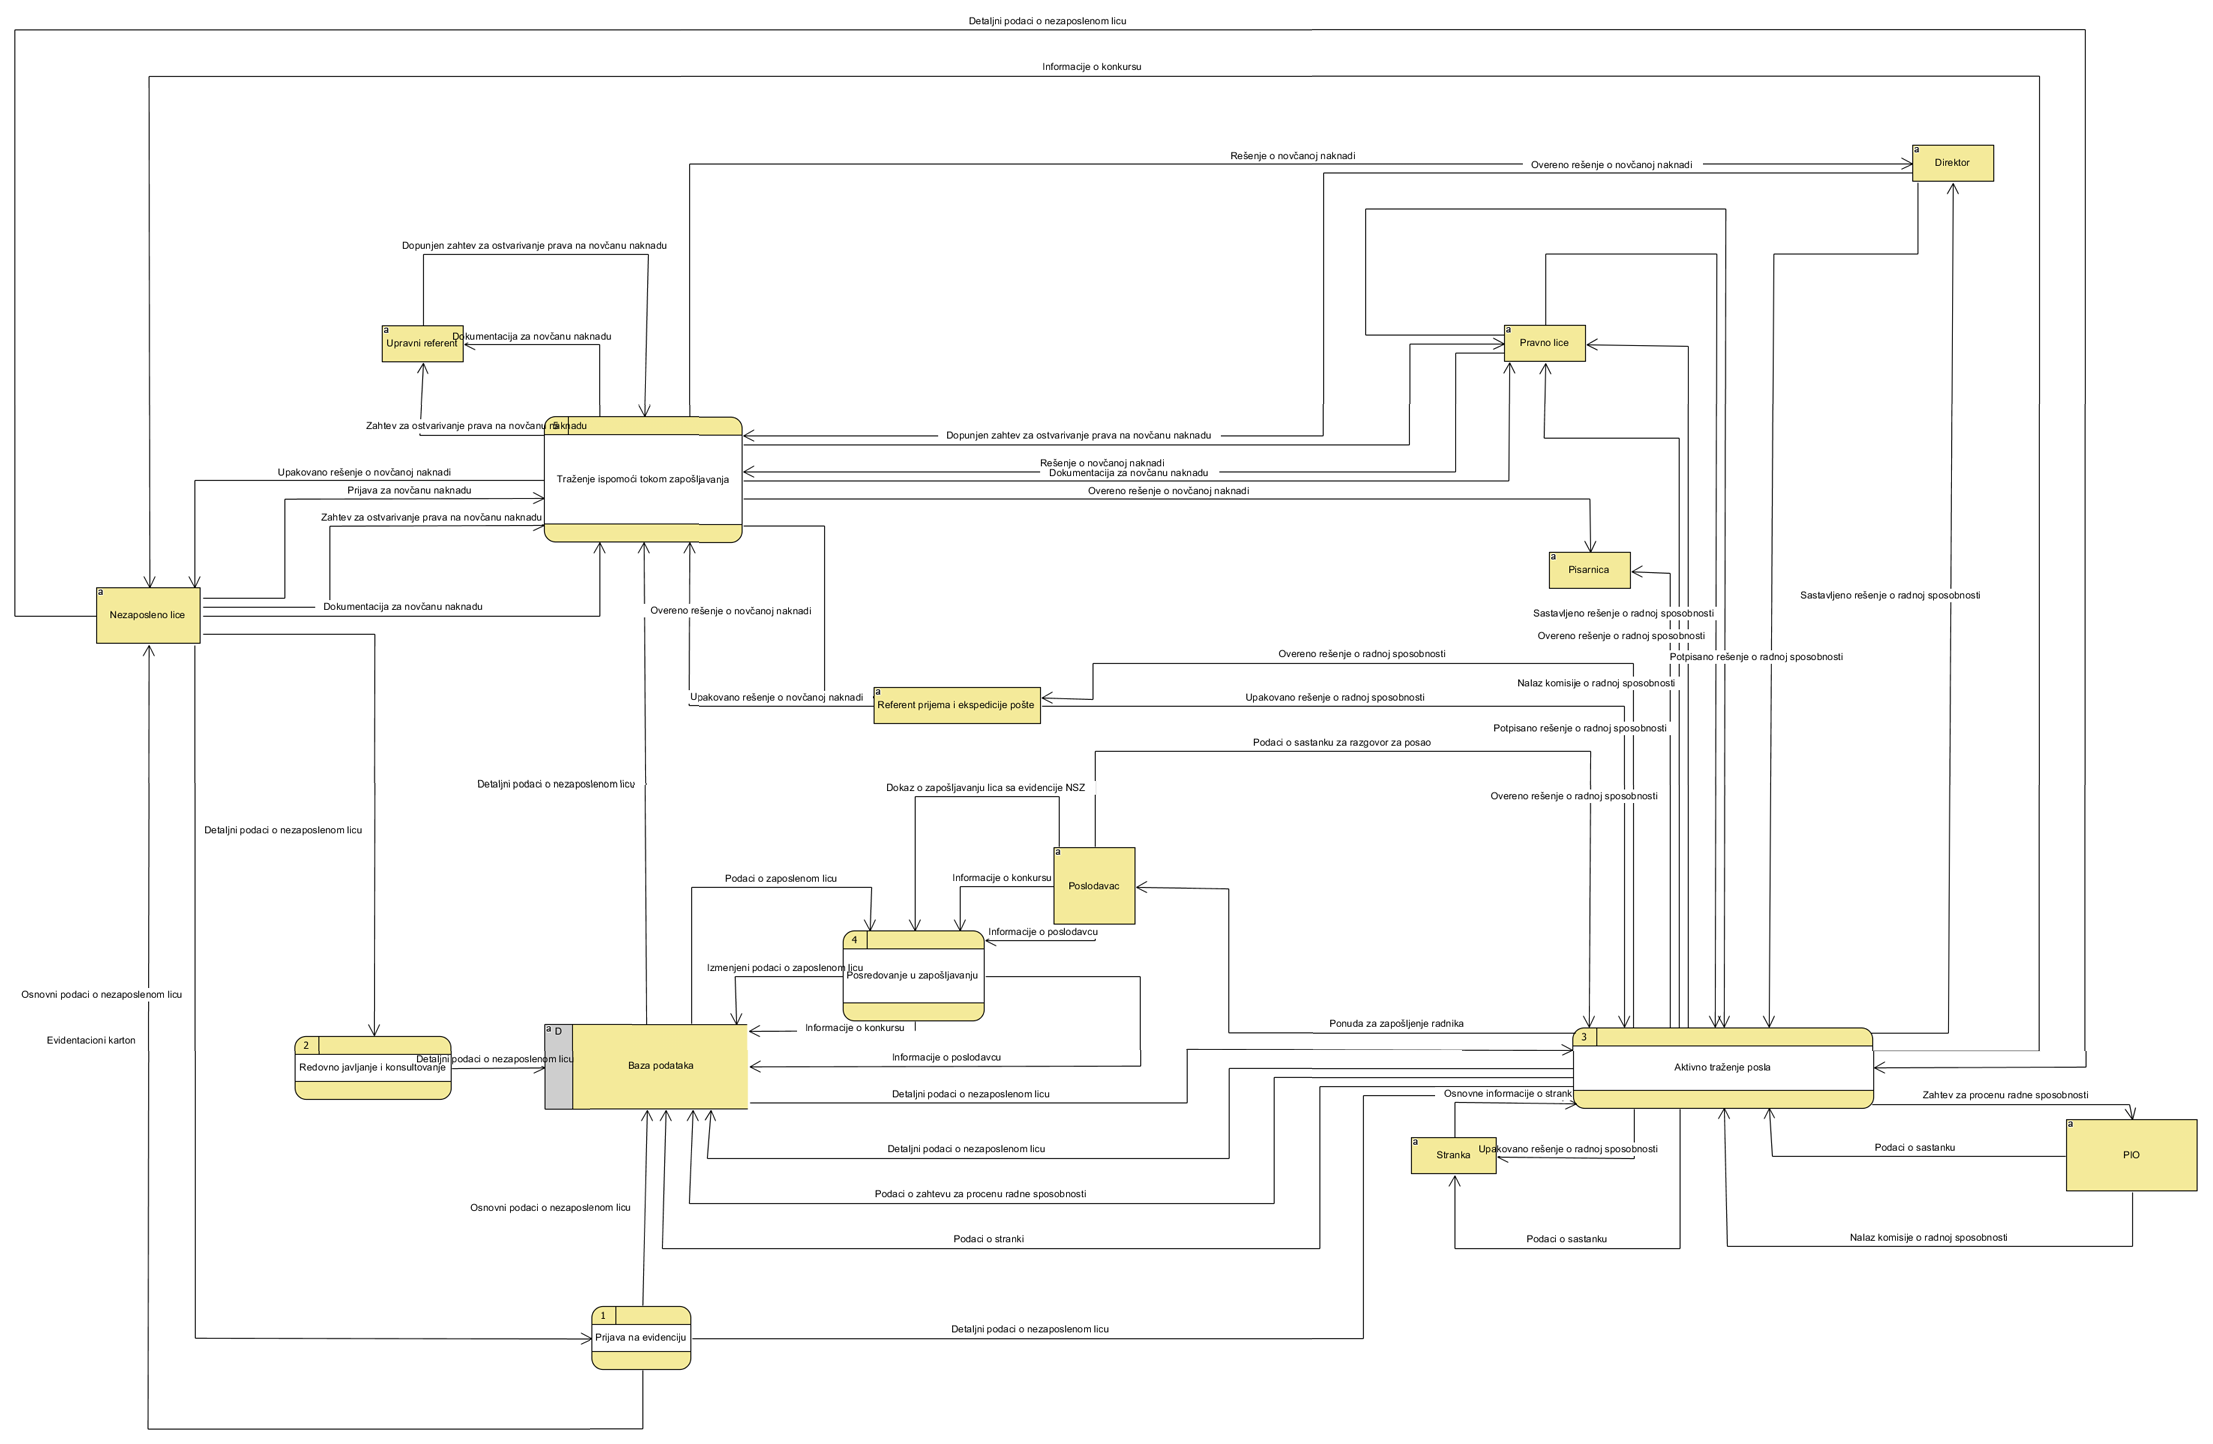
\includegraphics[width=0.7\paperwidth]{dijagrami/dijagrami-toka-podataka/zaposljavanje-dtp-nivoa-0.png}
		\caption{Dekompozicija procesa ''Zapo\v sljavanje'' (Slika \ref{dtp: dijagram konteksta}).}
	\end{figure}

\end{mylandscape}

\subsection{Metodologija rada}

Prilikom izrade rada, informacije o Nacionalnoj slu\v zbi su prikupljene iz dva glavna izvora. Prvi izvor predstavljaju zvani\v cna dokumenta Nacionalne slu\v zbe, i to ''Program rada Nacionalne slu\v zbe za zapo\v sljavanje (za 2016. godinu)'' i ''Statut Nacionalne slu\v zbe za zapo\v sljavanje'', \v cijim razmatranjem smo dolazili do formalnih informacija o sistemu. Drugi izvor informacija je razgovor sa zaposlenim licima, \v sto nam je prevashodno omogu\' cilo da steknemo uvid u mogu\' ca unapre\dj enja sistema.\\

Deo sistema koji je analiziran je modeliran kori\v s\' cenjem razli\v citih dijagramskih tehnika. U daljem tekstu \'cemo navesti kori\v s\'cene tehnike i dati ukratke opise.\\

Zahtevi sistema su modelirani dijagramima slu\v cajeva upotrebe (engl. \textit{Use Case Diagram}). Slu\v caj upotrebe je niz koraka pona\v sanja (scenario), automatskih i ru\v cnih, koji slu\v ze za kompletiranje jednog poslovnog zadatka. Dijagram slu\v cajeva upotrebe prikazuje interakciju izme\dj u sistema i eksternih sistema i korisnika. Drugim re\v cima, on grafi\v cki predstavlja ko \' ce koristiti sistem i na koje na\v cine korisnik mo\v ze da interaguje sa sistemom (\cite{SADM}). Dijagrami slu\v cajeva upotrebe su dopunjeni BPMN dijagramima i dijagramima sekvence.\\

\textit{Business Process Model and Notation} (skra\' ceno, BPMN) standard je za modeliranje poslovnih procesa koji obezbe\dj uje grafi\v cku notaciju za preciziranje poslovnih procesa. Cilj BPMN je da podr\v zi modeliranje poslovnih procesa za tehni\v cke i netehni\v cke (poslovne) korisnike nude\' ci notaciju koja je intuitivna poslovnim licima, a opet dovoljno jaka da mo\v ze da predstavi kompleksnu procesnu semantiku (\cite{BPMN}). Dakle, BPMN dijagrame (posebno, BPMN dijagrame saradnji) koristi\' cemo za opisivanje interakcije izme\dj u entiteta tokom slu\v cajeva upotrebe.\\

Dijagrami sekvence (engl. \textit{Sequence Diagram}) ilustruju objekte koji u\v cestvuju u slu\v caju upotrebe i poruke koje se razmenjuju izme\dj u njih u toku vremena, u jednom slu\v caju upotrebe (\cite{SAAD}). Ove dijagrame \' cemo koristiti pri slu\v cajevima upotrebe za koje smatramo da je potrebno dodatno opisati tok scenarija u vremenu.\\

Dijagram stanja (engl. \textit{state diagram} ili \textit{state machine diagram}) predstavlja dinami\v cki model koji prikazuje razli\v cita stanja kroz koje jedna klasa prolazi tokom svog \v zivota (\cite{SAAD}).\\

Dijagrami toka podataka (engl. \textit{Data Flow Diagrams}) predstavljaju jednu od osnovnih tehnika strukturnih metodologija. DTP opisuju na koji na\v cin se kre\' cu podaci kroz sistem. Razlikujemo nivoe DTP, pa tako dijagram konteksta predstavlja DTP najvi\v seg nivoa i njime se \v citav sistem (podsistem) predstavlja kao jedan proces (\cite{smalkov-slajdovi}). Dijagram konteksta \' cemo koristiti upravo da bismo pokazali granice sistema i komunikaciju sa njegovim okru\v zenjem.\\

Dijagram klasa (engl. \textit{Class Diagram}) predstavlja stati\v cki model koji podr\v zava stati\v cki pogled sistema u razvoju. On prikazuje klase i odnose izme\dj u klasa koje ostaju nepromenljive u sistemu tokom vremena (\cite{SAAD}).\\

Kao softversko re\v senje za izradu pomenutih dijagrama, kori\v s\' cen je Visual Paradigm 14.\\

Veliki broj opisanih slu\v cajeva upotrebe sadr\v zi rukovanje sa sistemom, pa zbog toga, u okviru ovog rada, obra\' cena je i pa\v znja na projektovanje korisni\v ckog interfejsa. Kao pristup izrade prototipa (engl. \textit{prototyping}) korisni\v ckog interfejsa odabran je HTML prototip.\\

HTML prototip se izgra\dj uje kori\v s\'cenjem Veb stranica napisanih u HTML (engl. \textit{HyperText Mark-up Language}) jeziku. Postupak podrazumeva kreiranje serije Veb stranica koje pokazuju fundamentalne delove sistema. Korisnici mogu da interaguju sa stranicama klikom na dugmad i uno\v senjem podataka u formulare (naravno, po\v sto nema sistema u pozadini, podaci se ne procesuiraju). Stranice su povezane tako da, kada korisnik klikne na dugmad, prikazuje se zahtevani deo sistema (\cite{SAAD}).

\newpage
\section{Slu\v cajevi upotrebe}

Slu\v caj upotrebe je celina posla koja daje nekakav smisleni rezultat, a dovoljno je mala da mo\v ze da se jednozna\v cno opi\v se i implementira \cite{smalkov-slajdovi}.\\

Opis slu\v caja upotrebe bi trebalo da bude dovoljno duga\v cak, tj. da obuhvati sve ono \v sto je potrebno da bi neko mogao na osnovu tog opisa da napravi ta\v cnu implementaciju. Svaki slu\v caj upotrebe mora da ima svoj opis \cite{smalkov-slajdovi}.\\

Ve\' cina UML dijagrama se zasniva prvenstveno na grafi\v ckom obliku. Dijagram slu\v cajeva upotrebe predstavlja odnose slu\v cajeva upotrebe i aktera. Pojedinosti slu\v cajeva upotrebe se opisuju tekstualno. Dobar opis slu\v caja upotrebe sadr\v zi dovoljno informacija da se mo\v ze sagledati kada, kako, ko i sa kojim podacima u\v cestvuje u slu\v caju upotrebe \cite{smalkov-slajdovi}.

\subsection{Prijava na evidenciju}

Nezaposleno lice dolazi li\v cno u Nacionalnu slu\v zbu za zapo\v sljavanje radi prijave na evidenciju. U zavisnosti od toga da li je lice ve\' c bilo na evidenciji ili ne razlikujemo dva slu\v caja:

\begin{itemize}
	\item ukoliko lice nije bilo nikada ranije prijavljeno na evideniciji, izvr\v sava se slu\v caj upotrebe Prva prijava (\ref{su: prva prijava})
	\item ukoliko je lice bilo prijavljeno na evidenciju ali je izgubilo status aktivnog tra\v zenja posla zbog neredovnog javljanja izvr\v sava se slu\v caj upotrebe Ponovna prijava (\ref{su: ponovna prijava}).
\end{itemize}

\begin{figure}[H]
	\centering
	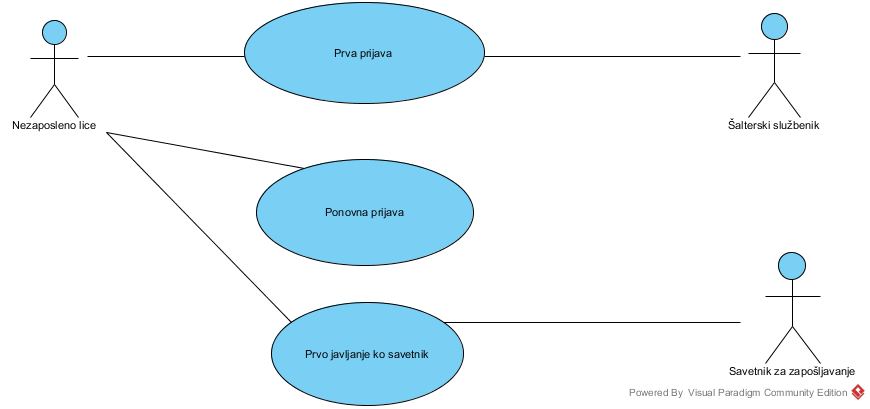
\includegraphics[width=0.8\textwidth]{dijagrami/dijagrami-slucajeva-upotrebe/prijava-na-evidenciju.png}
	\caption{Dijagram slu\v cajeva upotrebe - Prijava na evidenciju}
	\label{dsu: prijava na evidenciju}
\end{figure}

\subsubsection{Slu\v caj upotrebe: Prva prijava}
\label{su: prva prijava}

\noindent U\v cesnici: Nezaposleno lice (u daljem tekstu NL), \v salterski slu\v zbenik (u daljem tekstu \v SS)
\\
\\ Preduslovi: NL ima li\v cnu kartu i dokaz o stru\v cnoj spremi. Automat za izdavanje broja je u funkciji. \v SS je ulogovan na sistem. 
\\
\\ Postuslovi: NL je ili uspe\v sno prijavljen na evidenciju i izdat je evidencioni karton tra\v zioca zaposlenja, ili mu je ukazano na njegov status.
\\
\\ Glavni tok:
\begin{enumerate}
	\item NL prilazi automatu i bira opciju ''Prijava na evidenciju''.
	\item Automat bele\v zi da je opcija ''Prijava na evidenciju'' odabrana, ra\v cuna naredni broj u redu \v cekanja za tu opciju, i \v stampa papir sa brojem.
	\item NL uzima broj i \v ceka svoj red.
	\item Kada do\dj e na red, NL prilazi \v salteru i zahteva od \v SS da ga prijavi na evidenciju.
	\item \v SS otvara formular za prijavu.
	\item \v SS tra\v zi od NL da mu preda li\v cnu kartu i dokaz o stru\v cnoj spremi.
	\item NL predaje potrebna dokumenta. 
	\item \v SS popunjava formular na osnovu predatih dokumenata.
	\item \v SS daje NL-u da popuni Obrazac za prijavu na evidenciju.
	\item NL popunjava Obrazac za prijavu na evidenciju, a zatim ga vra\' ca \v SS-u.
	\item \v SS popunjava Evidencioni karton za tra\v zioca zaposlenja.
	\item \v SS zakazuje prvo javljanje savetniku za zapo\v sljavanje, i postavlja status NL-a na ''aktivan''.
	\item \v SS vra\' ca dokumenta NL-u i daje mu evidentacioni karton.
	\item Prelazi se na slu\v caj upotrebe \ref{su: prvo javljanje savetniku}.
\end{enumerate}

\noindent Alternativni tokovi: 
\begin{description}
	\item[A1. Pad sistema] ~\\
	Ukoliko se u bilo kom koraku Glavnog toka dogodi pad sistema na kojem radi \v SS, \v SS ponovo pokre\'ce sistem i prijavljuje se na njega.
	\begin{enumerate}
		\item \v SS proverava da li je formular sa\v cuvan.
		\item Ukoliko jeste, prelazi se na korak 9 Glavnog toka.
		\item Ina\v ce, prelazi se na korak 8 Glavnog toka.
	\end{enumerate}

	\item[A2. Status NL-a je ''zamrznut''] ~\\
	Ukoliko u koraku 8 Glavnog toka sistem prika\v ze da postoje informacije o NL-u, kao i da je njegov status ''zamrznut'', \v SS obave\v stava NL-a o njegovom statusu, i slu\v caj upotrebe se zavr\v sava.
\end{description}

\subsubsection{Slu\v caj upotrebe: Ponovna prijava}
\label{su: ponovna prijava}

\noindent  U\v cesnici: Nezaposleno lice (u daljem tekstu NL), \v salterski slu\v zbenik (u daljem tekstu \v SS)
\\
\\ Preduslovi: NL ima li\v cnu kartu. Automat za izdavanje broja je u funkciji. \v SS je ulogovan na sistem. 
\\
\\ Postuslovi: NL-u je uspe\v sno promenjen status i izdat je novi evidencioni karton tra\v zioca zaposlenja.
\\
\\ Glavni tok:
\begin{enumerate}
	\item NL prilazi automatu i bira opciju ''Prijava na evidenciju''.
	\item Automat bele\v zi da je opcija ''Prijava na evidenciju'' odabrana, ra\v cuna naredni broj u redu \v cekanja za tu opciju, i \v stampa papir sa brojem.
	\item NL uzima broj i \v ceka svoj red.
	\item Kada do\dj e na red, NL prilazi \v salteru i zahteva od \v SS da mu promeni status.
	\item \v SS tra\v zi od NL da mu preda li\v cnu kartu.
	\item NL predaje li\v cnu kartu.
	\item \v SS pronalazi NL-a u sistemu. 
	\item \v SS bira opciju izmeni podatke.
	\item \v SS menja status "zamrznut" u "aktivan".
	\item \v SS popunjava Evidencioni karton za tra\v zioca zaposlenja.
	\item \v SS zakazuje prvo javljanje savetniku za zapo\v sljavanje, i postavlja status NL-a na ''aktivan''.
	\item \v SS vra\' ca dokumenta NL-u i daje mu evidentacioni karton.
	\item Prelazi se na slu\v caj upotrebe \ref{su: prvo javljanje savetniku}.
\end{enumerate}

\noindent Alternativni tok: /

\subsubsection{Slu\v caj upotrebe: Prvo javljanje savetniku}
\label{su: prvo javljanje savetniku}

\noindent U\v cesnici: Nezaposleno lice (u daljem tekstu NL), savetnik za zapo\v sljavanje (SZ)
\\
\\ Preduslovi: NL ima evidentacioni karton. SZ je ulogovan na sistem. 
\\
\\ Postuslovi: Ili je uspe\v sno zabele\v zeno javljanje NL-a ili je postavljen status NL-a na ''zamrznut''.
\\ 
\\ Glavni tok:
\begin{enumerate}
	\item NL dolazi kod SZ-a u kancelariju i predaje mu svoj evidentacioni karton.
	\item SZ pronalazi NL-a u sistemu.
	\item SZ i NL razgovaraju o NL-ovoj stru\v cnoj spremi, kakvi poslovi zanimaju NL-e, i koje ve\v stine Nl poseduje.
	\item SZ unosi nove informacije u sistem.
	\item SZ tra\v zi informacije o prethodnim zaposlenjima NL-a, i ako postoje i te informacije, SZ ih unosi u sistem.
	\item SZ zakazuje slede\' ce javljanje i vra\' ca NL-u evidentacioni karton.
\end{enumerate}

\noindent Alternativni tok:
\begin{description}
	\item[A1. Promena statusa NL-a na ''zamrznut''] ~\\
	Ukoliko u koraku 1 Glavnog toka NL ne do\dj e na prvo javljanje pre zakazanog termina, automatski se \v salje zahtev za izmenom podataka o NL-u u sistemu, i to: status NL-a se prebacuje na ''zamrznut''. Slu\v caj upotrebe se zavr\v sava.
\end{description}
\subsection{Redovno javljanje}

Redovno javljanje predstavlja postupak dolaska nezaposlenog lica u Nacionalnu slu\v zbu radi vo\dj enja redovne evidencije o teku\' cem stanju. Nezaposleno lice je u obavezi da se na svaka 3 meseca javi u Nacionalnoj slu\v zbi, i da izvesti zaposlene koji posreduju u zapo\v sljavanju o svom trenutnom statusu.\\

U zavisnosti od nivoa izve\v stavanja nezaposleno lice mo\v ze da bira na\v cin redovnog javljanja, i to:
\begin{itemize}
	\item ukoliko nema potrebu za dodatnim uslugama Nacionalne slu\v zbe, bira jedno od naredna dva:
	\begin{itemize}
		\item Javljanje na \v salteru (slu\v caj upotrebe \ref{su: javljanje na salteru}), ili
		\item Javljanje putem interneta (slu\v caj upotrebe \ref{su: javljanje putem interneta}).
	\end{itemize}
	
	\item ukoliko ima potrebu za dodatnim uslugama Nacionalne slu\v zbe, onda bira Javljanje kod savetnika (slu\v caj upotrebe \ref{su: javljanje kod savetnika}).
\end{itemize}

Unapre\dj enje trenutnog re\v senja predstavlja Javljanje putem interneta. Ovim slu\v cajem upotrebe se uvodi novi deo onlajn sistema Nacionalne slu\v zbe, radi olak\v savanja procesa Redovno Javljanje nezaposlenih lica koji nemaju dodatne potrebe za uslugama Nacionalne slu\v zbe. Doprinosi ovog unapre\dj enja su:
\begin{itemize}
	\item smanjenje reda \v cekanja u Nacionalnoj slu\v zbi,
	\item usmeravanje rada \v salterskog slu\v zbenika na druge (zna\v cajnije) radne aktivnosti i zadatke, i
	\item obavljanje procesa Redovno javljanje iz komfornosti doma.
\end{itemize}

\subsubsection{Javljanje na \v salteru}
\label{su: javljanje na salteru}

\noindent U\v cesnici: Nezaposleno lice (u daljem tekstu NL), \v salterski slu\v zbenik (u daljem tekstu \v SS)
\\
\\ Preduslovi: NL ima evidentacioni karton. \v SS je ulogovan na sistem. 
\\
\\ Postuslovi: Ili je uspe\v sno zabele\v zeno javljanje NL-a ili je NL obave\v sten o svom stanju.
\\ 
\\ Glavni tok:
\begin{enumerate}
	\item NL prilazi automatu i bira opciju ''Redovno javljanje''.
	\item Automat bele\v zi da je opcija ''Redovno javljanje'' odabrana, ra\v cuna naredni broj u redu \v cekanja za tu opciju, i \v stampa papir sa brojem.
	\item NL uzima broj i \v ceka svoj red.
	\item Kada do\dj e na red, NL prilazi \v salteru, zahteva od \v SS da prijavi njegov dolazak, i predaje \v SS-u svoj evidentacioni karton.
	\item \v SS pronalazi NL-a u sistemu.
	\item \v SS unosi u sistem da je NL do\v sao na redovno javljanje.
	\item \v SS zakazuje slede\' ce javljanje i vra\' ca NL-u evidentacioni karton.
\end{enumerate}

\noindent Alternativni tokovi: 
\begin{description}
	\item[A1. Pad sistema] ~\\
	Ukoliko se u bilo kom koraku Glavnog toka dogodi pad sistema na kojem radi \v SS, \v SS ponovo pokre\'ce sistem i prijavljuje se na njega. Prelazi se na korak 5 Glavnog toka.
	
	\item[A2. Status NL-a je ''zamrznut''] ~\\
	Ukoliko u koraku 5 Glavnog toka sistem prika\v ze da je status NL-a ''zamrznut'', \v SS obave\v stava NL-a o njegovom statusu, i slu\v caj upotrebe se zavr\v sava.
\end{description}

\subsubsection{Javljanje putem interneta}
\label{su: javljanje putem interneta}

\subsubsection{Javljanje kod savetnika}
\label{su: javljanje kod savetnika}

\begin{thebibliography}{9}
	
	\bibitem{smalkov-slajdovi}
	Malkov Sa\v sa.
	\href{http://poincare.matf.bg.ac.rs/~smalkov/nastava.master.html\#r271\_is}{\textit{Slajdovi sa predavanja na kursu Informacioni sistemi}}.
	
\end{thebibliography}

\end{document}